\chapter{Tendermint Consensus}
\label{ch:tendermint}

This chapter presents the Tendermint algorithm for consensus 
and an associated blockchain for atomic broadcast.
The BFT consensus problem is described in detail, 
and a formal specification of Tendermint consensus is given in the $\pi$-calculus.
The Tendermint blockchain is informally proven to satisfy atomic broadcast,
following the original proof of safety for Raft.
We leave it to future work to capture the full blockchain protocol in 
a process calculus and to verify its properties.

\section{Tendermint Overview}

Tendermint is a secure state-machine replication algorithm in the blockchain paradigm.
It provides a form of BFT-ABC that is furthermore accountable - 
if safety is violated, it is always possible to verify who acted maliciously.

Tendermint begins with a set of \emph{validators}, identified by their public key,
where each validator is responsible for maintaining a full copy of the replicated state,
and for proposing new blocks (batches of transactions), and voting on them.
Each block is assigned an incrementing index, or \emph{height}, 
such that a valid blockchain has only one valid block at each height.
At each height, validators take turns proposing new blocks in \emph{rounds}, 
such that for any given round there is at most one valid proposer.
It may take multiple rounds to commit a block at a given height due to the asynchrony of the network,
and the network may halt altogether if more than one-third of the validators are offline or partitioned.
Validators engage in two phases of voting on a proposed block before it is committed, 
and follow a simple locking mechanism which prevents any coalition of up to 
one third malicious validators from compromising safety.

Note that the core round-based voting mechanism is the consensus algorithm, 
which is strung together into blocks to yield atomic broadcast.
Each block contains some metadata, known as its \emph{header}, 
which includes the hash of the block at the previous height, resulting in a hash chain.
The header also includes the block height, local time the block was proposed, 
and the Merkle root hash of transactions included in the block.

\section{Consensus}

The consensus algorithm can be roughly divided into the following, somewhat orthogonal, components:

\begin{itemize}

\item{Proposals: a new block must be proposed by the correct proposer at each round, and gossiped to the other validators. If a proposal is not received in sufficient time, the proposer should be skipped.}

\item{Votes: two phases of voting must occur to ensure optimal Byzantine fault tolerance. They are called \emph{pre-vote} and \emph{pre-commit}. $A$ set of pre-commits from more than two-thirds of the validators for the same block at the same round is a \emph{commit}.}

\item{Locks: Tendermint ensures that no two validators commit a different block at the same height, presuming less than one-third of the validators are malicious. This is achieved using a locking mechanism which determines how a validator may pre-vote or pre-commit depending on previous pre-votes and pre-commits at the same height. Note that this locking mechanism must be carefully designed so as to not compromise liveness.}

\end{itemize}

\begin{figure}[]
	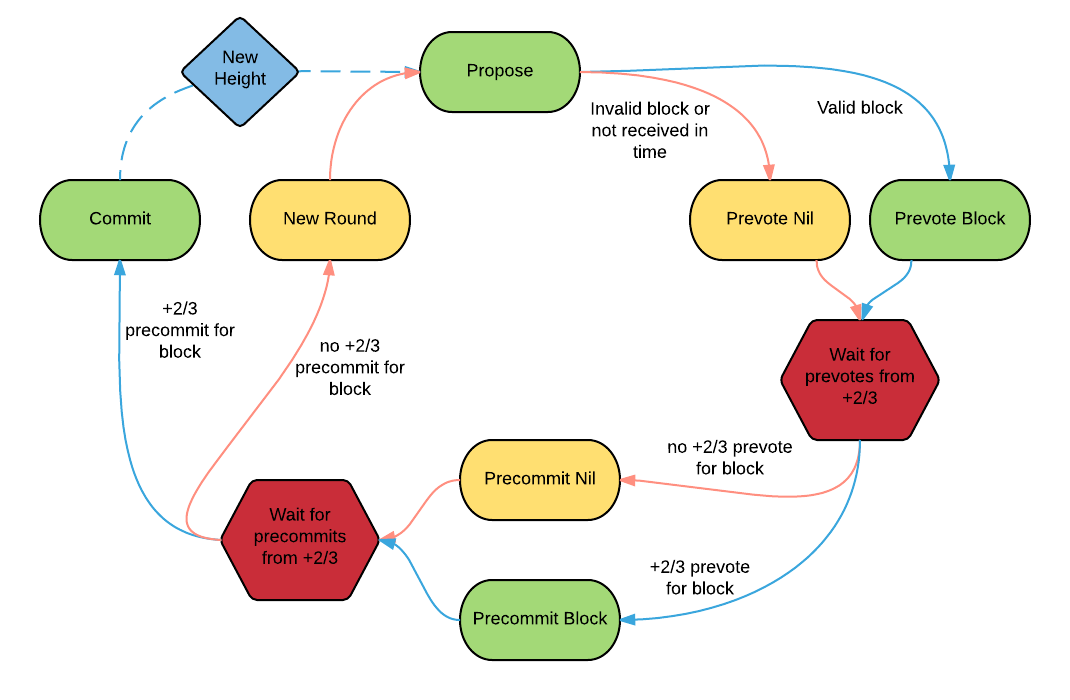
\includegraphics[width=\linewidth,height=\textheight,keepaspectratio]{figures/diagrams/consensus_logic.png}
    	\centering
	\caption[Overview of Tendermint consensus logic]{
After the proposal step, validators only make progress after hearing from two-thirds or more (+2/3) of other validators. The dotted arrow extends the consensus into atomic broadcast by moving to the next height.}
	\label{fig:consensus_logic}
\end{figure}

In order to provide tolerance to a single Byzantine fault, 
a Tendermint network must contain at minimum four validators.
Each validator must possess an asymmetric cryptographic key-pair for producing digital signatures.
Validators start from a common initial state, 
which contains the ordered list, $\mathcal{L}$, of validators.
Each validator is identified via their public key, and 
all proposals and votes must be signed by the respective private key.
This ensures that proposals and votes can always be verified by any observer.
It is helpful to assume that up to one-third of validators are malicious, 
co-operating in arbitrary ways to subvert system safety or liveness.

Consensus begins at round 0; the first proposer is the first validator in $\mathcal{L}$.
The outcome of a round is either a commit, or a decision to move to the next round.
With a new round comes the next proposer.
Using multiple rounds gives validators multiple opportunities 
to come to consensus in the event of network asynchrony or validator failures.

In contrast to algorithms which require a form of leader election, 
Tendermint has a new leader (the proposer) for each round.
Validators vote to skip to the next round in the same way they vote to accept the proposal,
lending the protocol a uniformity of mechanism that is absent 
from algorithms with an explicit leader-election program.

The beginning of each round has a weak dependence on synchrony as it utilizes local clocks to determine when to skip a proposer.
That is, if a validator does not receive a proposal within a locally measured \emph{TimeoutPropose} of entering a new round, it can vote to skip the proposer.
Inherent in this mechanism is the assumption that, at least eventually, the proposal will be delivered within \emph{TimeoutPropose}, which may itself increment with each round.
This assumption is discussed more fully in Chapter \ref{ch:related}.

After the proposal, rounds proceed in a fully asynchronous manner - a validator makes progress only after hearing from more than two-thirds of the other validators.
This relieves any sort of dependence on synchronized clocks or bounded network delays,
but implies that the network will halt if one-third or more of the nodes become unresponsive.
This circuit of weakly synchronous proposals, followed by asynchronous voting, 
is depicted in Figure \ref{fig:consensus_logic}.

To round-skip safely, a small number of \emph{locking} rules 
are introduced which force validators to justify their votes.
While we don't necessarily require them to broadcast their justifications in real time, 
we do expect them to keep the data,
such that it can be brought forth as evidence in the event that safety 
is compromised by sufficient Byzantine failures.
This accountability mechanism enables Tendermint to provide 
stronger guarantees in the face of such failure than eg.~PBFT,
which provides no guarantees if a third or more of the validators are Byzantine.

Validators communicate using a diverse set of messages for managing the blockchain, 
application state, peer network, and consensus.
The core consensus algorithm, however, consists of just two messages:

\begin{itemize}
\item{\emph{ProposalMsg}: a proposal for a block at a given height and round, signed by the proposer.}
\item{\emph{VoteMsg}: a signed vote for a proposal.}
\end{itemize}

In practice, we use additional messages to optimize the gossiping of block data and votes, as discussed in Chapter \ref{ch:subprotocols}.

\subsection{Proposals}

Each round begins with a proposal. 
The propser for the given round takes a batch of recently received transactions from its local cache (the Mempool, see Chapter \ref{ch:subprotocols}),
composes a block, and broadcasts a signed ProposalMsg containing the block.
If the proposer is Byzantine, it might broadcast different proposals to different validators.

Proposers are ordered via a simple, deterministic round robin, 
so only a single proposer is valid for a given round, 
and every validator knows the correct proposer. 
If a proposal is received for a lower round, or from an incorrect proposer, it is rejected.

Cycling of proposers is necessary for Byzantine tolerance. 
For instance, in Raft, if an elected leader is Byzantine and maintains strong network connections to other nodes,
it can completely compromise the system, destroying all safety and liveness guarantees.
Tendermint preserves safety via the voting and locking mechanisms, 
and maintains liveness by cycling proposers, so if one won't process any transactions, others can pick up.
Perhaps more interestingly, validators can vote through governance modules (see Chapter \ref{ch:governance}) to remove or replace Byzantine validators.

\subsection{Votes}

Once a complete proposal is received by a validator, 
it signs a pre-vote for that proposal and broadcasts it to the network.
If a validator does not receive a correct proposal within \emph{ProposalTimeout}, 
it prevotes for \emph{nil} instead.

In asynchronous environments with Byzantine validators, 
a single stage of voting, where each validator casts only one vote,
is not sufficient to ensure safety.
In essence, because validators can act fraudulently, 
and because there are no guarantees on message delivery time,
a rogue validator can co-ordinate some validators to commit a value
while others, having not seen the commit, 
go to a new round, within which they commit a different value.

A single round of voting allows validators to tell each other what they know about the proposal.	
But to tolerate Byzantine faults (which amounts, essentially to lies, fraud, deceipt, etc.), 
they must also tell each other what they know about what other validators have professed to know about the proposal.
In otherwords, a second stage ensures that enough validators witnessed the result of the first stage.

A pre-vote for a block is thus a vote to prepare the network to commit the block.
A pre-vote for nil is a vote to prepare the network to move to the next round.
In an ideal round with an online proposer, more than two-thirds of validators will pre-vote for the proposal.
A set of more than two-thirds of pre-votes for a single block at a given round is known as a \emph{polka}\footnote{The original term used was PoL, or PoLC, for Proof-of-Lock or Proof-of-Lock-Change. The term evolved to polka as it was realized the validators are doing the polka.}.
A set of more than two-thirds of pre-votes for nil is a \emph{nil-polka}

When a validator receives a polka (read: more than two-thirds pre-votes for a single block), 
it has received a signal that the network is prepared to commit the block,
and serves as justification for the validator to sign and broadcast a pre-commit vote for that block.
Sometimes, due to network asynchrony, a validator may not receive a polka, or there may not have been one. 
In that case, the validator is not justified in signing a pre-commit for that block, 
and must therefore sign and publish a pre-commit vote for nil.
That is, it is considered malicious behaviour to sign a pre-commit without justification from a polka.

A pre-commit is a vote to actually commit a block.
A pre-commit for nil is a vote to actually move to the next round.
If a validator receives more than two-thirds pre-commits for a single block, 
it commits that block, computes the resulting state,
and moves on to round 0 at the next height.
If a validator receives more than two-thirds nil-pre-commits,
it moves on to the next round.

\subsection{Locks}

Ensuring safety across rounds can be tricky, 
as circumstances must be avoided which would provide justification for two different blocks to be committed at two different rounds at the same height.
In Tendermint, this problem is solved via a \emph{locking} mechanism.
In essence, once a pre-commit is cast, a validator is \emph{locked} on the associated block, and must follow certain locking rules.
There are two rules of locking:

\begin{itemize}
\item{Prevote-the-Lock: a validator must pre-vote for the block they are locked on,
	and propose it if they are the proposer.	
	This prevents validators from pre-committing one block in one round, 
	and then contributing to a polka for a different block in the next round, 
	thereby compromising safety.}
\item{Unlock-on-Polka: a validator may only release a lock after seeing a polka at a round greater than that at which it locked.
	This allows validators to unlock if they pre-committed something the rest of the network doesn't want to commit,
	thereby protecting liveness, but does it in a way that does not compromise safety,
	by only allowing unlocking if there has been a polka in a round after that in which the validator became locked.}
\end{itemize}


For simplicity, a validator is considered to have locked on nil at round -1 at each height, 
so that Unlock-on-Polka implies that a validator cannot precommit at all at a new height until they see a polka.

These rules can be understood more intuitively by way of examples. 
Consider four validators, $A$, $B$, $C$, $D$, and suppose there is a proposal for $blockA$ at round $R$. 
Suppose there is a polka for $blockX$, 
but $A$ doesn't see it, and precommits nil, 
while the others precommit for $blockX$.
Now suppose the only one to see all precommits is D, 
while the others, say, don't see D's precommit (they only see their two precommits and Val1's nil-precommit).
D will now commit the block, while the others go to round $R+1$.
Since any of the validators might be the new proposer, 
if they can propose and vote for any new block, say $blockY$, 
then they might commit it and compromise safety, since $D$ already committed $blockA$.
Note that there isn't even any Byzantine behaviour here, just asynchrony!

Locking solves the problem by forcing validators to stick with the block they pre-committed, 
since other validators might have committed based on those precommits (as $D$ did in this example).
In essence, once more than two-thirds precommit a block in a round, the network is locked on that block,
which is to say it must be impossible to produce a valid polka for a different block at a higher round.
This is direct motivation for Prevote-the-Lock.

Prevote-the-Lock is not sufficient, however. 
There must be a way to unlock, lest we sacrifice liveness.
Consider a round where $A$ and $B$ precommitted $blockX$ while $C$ and $D$ precommitted nil - a split vote.
They all move to the next round, and $blockY$ is proposed, which $C$ and $D$ prevote for.
Suppose $A$ is Byzantine, and prevotes for $blockY$ as well (despite being locked on $blockX$), resulting in a polka.
Suppose $B$ does not see the polka and precommits nil, while $A$ goes off-line and $C$ and $D$ precommit $blockY$. 
They move to the next round, but $B$ is still locked on $blockX$, while $C$ and $D$ are now locked on $blockY$, 
and since $A$ is offline, they can never get a polka. 
Hence, we've compromised liveness with less than a third (here, only one) Byzantine validators.

The obvious justification for unlocking is a polka. 
Once $B$ sees the polka for $blockY$ (which $C$ and $D$ used to jusitfy their precommits for $blockY$), 
it ought to be able to unlock, and hence precommit $blockY$.
This is the motivation for Unlock-on-Polka, 
which allows validators to unlock (and precommit a new block),
if they have seen a polka in a round greater than that in which they locked.

\subsection{Formal Specification}

Now that we have explained the protocol in detail, 
we provide a formal specification in the $\pi$-calculus.

Let $Consensus := \prod_{i=1}^N Y_i $ represent a consensus protocol
over a set of $N$ validators, each executing one of a mutually exclusive set of processes, $Y_i$.
Internal state $s = \{r, p, v \}$ consists of a strictly increasing round, $r$,
a proposal $p$, containing the proposed block for this round;
and a set of votes, $v$, containing all votes at all rounds;
We denote by $v_r^1$ and $v_r^2$ the set of prevotes and precommits, respectively, at round $r$.
We define $proposer(r) = r \mod n$ to be the index of the proposer at round $r$.
We represent a peer at a particular point in the protocol as $Y_i^{r, p, v}$.
Processes $Y_i$ range over $PR_i$, $PV_i$, $PC_i$, $C_i$,
respectively abbreviating 
\emph{propose}, \emph{prevote}, \emph{precommit}, \emph{commit}.
We introduce additional sub-functions for $PV$ and $PC$ to capture the recursion,
denoted $PV1$, $PV2$, etc.

Peers are connected using broadcast channels for each message type,
namely $propose_i$, $prevote_i$, and $precommit_i$,
as well as a channel for broadcasting new transactions, $b_i$,
and one for deciding on, or committing, the next block, $d_i$.
Via an abuse of notation, a single send on some $x_i$ can be received by each process along
$x_i$.

We use only two message types: proposals and votes. 
Each contains a round number, block (hash), and signature, 
denoted $msg.round$, $msg.block$, $msg.sig$.
Note we can absorb the signature into the broadcast channel itself,
but we need it for use as evidence in the event of byzantine behaviour.

The specification is given in Figure \ref{fig:tendermint-pi}

\begin{figure}[]
	
\begin{center}
	\begin{tabular}{l }
		\hline \\
		$Consensus := \prod_{i=1}^N [ PR_i^{0,\emptyset,\emptyset,} \| D_i]$ \\\\

		\hline \\
		{$\!\begin{aligned}
		PR_i^{r,p,v} := 
			& \text{if } i=proposer(r) \text{ then } \\
				& \quad propose_i ! (prop) \| PV_i^{r,prop,v} \text{, where } prop = chooseProposal(p)\\
			& \text{ else if } p \neq \emptyset \text{ then}  \\
				& \quad PV_i^{r,p,v}  \\
			& \text{else} \\ 
				& \quad propose_{proposer(r)} ? (prop).PV_i^{r,prop,v} + susp_{proposer(r)}.PV_i^{r,\emptyset,v} \\
		\end{aligned}$} \\\\

		\hline \\
		$PV_i^{r,p,v}:= prevote_i ! (r,p) \| (\nu \> c) ( \prod_{j=1}^n prevote_j ? (w) . c!(w)  \| PV1_i^{r,p,v}(c))$ \\\\

		\hline \\
		{$\!\begin{aligned}
		PV1_i^{r,p,v}(c) := 
			& \text{ if } max_{b}(|\left\{ w \in v_r^1 : w.block = b\right\}|) > \frac{2}{3} N \text{ then} \\
				& \quad PC_i^{r,b,v} \\
			& \text{else if }  | v_r^1 | > \frac{2}{3} N \text{ then} \\ 
				& \quad PC_i^{r,\emptyset,v} \\ 
			& \text{else} \\
				& \quad c?(vote) . PV1_i^{r,p,vote::v}(c) \\
		\end{aligned}$} \\\\

		\hline \\
		$PC_i^{r,p,v}:= precommit_i ! (r,p) \| (\nu \> c) ( \prod_{j=1}^n precommit_j ? (w) . c!(w)  \| PC1_i^{r,p,v}(c))$ \\\\

		\hline \\
		{$\!\begin{aligned}
		PC1_i^{r,p,v}(c) := 
			& \text{ if } max_{b}(|\left\{ w \in v_r^2 : w.block = b\right\}|) > \frac{2}{3} N \text{ then} \\
				& \quad C_i^{r,b,v} \\
			& \text{else if }  | v_r^2 | > \frac{2}{3} N \text{ then} \\ 
				& \quad PR_i^{r+1,\emptyset,v} \\ 
			& \text{else} \\
				& \quad c?(vote) . PC1_i^{r,p,vote::v}(c) \\
		\end{aligned}$}


	\end{tabular}
\end{center}


	\label{fig:tendermint-pi}
\end{figure}

\section{Blockchain}

Tendermint operates on batches (blocks) of transactions at a time.
Continuity is maintained from one block to the next by explicitly linking each block to the one before it 
via it's cryptographic hash, forming a blockchain. 
The blockchain contains the ordered transaction log and evidence that the block was committed 
by the validators.

\subsection{Why Blocks?}
Consensus algorithms typically commit transactions one at a time by design, 
and implement batching after the fact.
As mentioned in Chapter \ref{ch:background}, 
tackling the problem from the perspective of batched atomic broadcast
results in two primary optimizations, which give us more throughput and fault-tolerance:

\begin{itemize}
\item{Bandwidth optimization: since every commit requires two rounds of communication across all validators, 
	batching transactions in blocks amortizes the cost of a commit over all the transactions in the block.}
\item{Integrity optimization: the hash chain of blocks forms an immutable data structure, much like a Git repository, enabling authenticity checks for sub-states at any point in the history.}
\end{itemize}

Blocks induce another effect as well, which is more subtle but potentially important. 
They increase the minimum latency of a transaction to that of the whole block, 
which for Tendermint is on the order of hundreds of milliseconds to seconds.
Traditional serializable database systems provide commit latencies on the 
order of milliseconds to tens of milliseconds.
They are able to do this because they are not Byzantine Fault Tolerant, 
requiring only one round of communication (instead of two)
and responses from over half of the replicas (instead of two-thirds).
However, unlike the fast commit times interrupted by leader elections in other algorithms,
Tendermint provides a more regular pulse that is more responsive to the overall health of the network, 
in terms of node failures and asynchrony.

What role such pulses might play in the coherence of 
communicating autonomous systems on the internet is yet to be determined,
though purposefully induced latency has shown promise in the financial markets \cite{iex}.

\subsection{Block Structure}

The purpose of blocks is to contain a batch of transactions, and to link to the previous block.
The link comes in two forms: the previous block hash,
and the set of pre-commits which caused the previous block to be committed, also known as the $LastCommit$.
Thus a block is composed of three parts: the block header, the list of transactions, and the $LastCommit$.
The composition of the header is given in Figure \ref{fig:header}

\begin{figure}[]
	
\begin{verbatim}
type Header struct {
	ChainID            string        
	Height             int           
	Time               time.Time     
	NumTxs             int           
	LastBlockHash      []byte        
	LastBlockParts     PartSetHeader 
	LastCommitHash []byte       // Merkle root hash of LastCommit
	DataHash           []byte   // Merkle root hash of transaction 
	ValidatorsHash     []byte   // Merkle root hash of validator set
	AppHash            []byte   // state Merkle root from previous block's transactions
}

type PartSetHeader struct {
	Total int    
	Hash  []byte 
}
\end{verbatim}
	\caption[Block Header Structure]{The fields required for a valid block header. The validity of all fields is checked before pre-commit}

	\label{fig:header}
\end{figure}

\section{Safety}

Here we sketch a brief proof of Tendermint's safety guarantee, namely, 
the State Machine Safety property, that for two validators to apply different blocks at the same height
requires at least one-third of valdiators to be Byzantine.

Referring back to the safety guarantees in Figure \ref{fig:tendermint_guarantees}, 
note that Proposer Safety, Validator Append Only, and Proposer Completeness are trivially satisfied by the protocol, 
in particular through the use of a round-robin for the proposer selection and hash links to connect blocks,
and by not allowing blocks to be overwritten.

Suppose that two blocks are committed at the same height.
Let the blocks be $blockA$ and $blockB$, and let them be committed in rounds $R_A$ and $R_B$, respectively, with $R_A < R_B$.
Since each commit requires more than two-thirds of validators, 
two commits requires that more than a third of validators sign for both commits.
Let this set of validators be $D$.
Note that if $R_A = R_B$, a single proposer must have proposed two blocks at the same round, 
and the validators in $D$ must have precommitted for both $blockA$ and $blockB$ in that same round, 
making the proof trivial, since double signing within a round is Byzantine.

With blocks committed in different rounds, however, 
we must show that at least a third of validators violated the locking rules.
We already know that the validators from $D$ lock on $blockA$ in $R_A$.
To unlock from $blockA$, and precommit for $blockB$, 
they must observe a polka for $blockB$ at round $R_P$, where $R_A < R_P <= R_B$.
A polka requires more than two-thirds of validators to prevote for the same block.
Since more than two-thirds locked on $blockA$ at round $R_A$, 
a polka for a different block at a higher round requires more than a third to violate Prevote-the-Lock.
Given Proposer Safety, Validator Append Only, and Proposer Completenes,
this guarantees State Machine Safety assuming less than one-third of validators are Byzantine.

In future work, we aim to provide a more formal proof of Tendermint's correctness 
and the ability to identify validators which violated locking rules.


%
%- Proposer Safety condition implied by protocol
%- Validator Append Only condition implied by the protocol
%- Proposer Completeness guaranteed by the merkle hash chain
%
%Need to show Block Matching, State Machine Safety, and Deterministic Accountability.
%Locking rules give us lemmas about polkas.
%


\section{Faults and Availability}

As a BFT consensus algorithm, Tendermint can tolerate Byzantine failure in up to (but not including) one-third of validators.
This means nodes can crash, send different and contradictory messages to different peers, refuse to relay messages, or otherwise behave arbitrarily,
without compromising safety or liveness (with the usual FLP caveat for liveness).

There are two places in the protocol where we can make optimizations for asynchrony by utilizing timeouts based on local clocks:
after receiving two-thirds or more pre-votes, but not for a single block or nil, and after receiving two-thirds or more pre-commits, 
but not for a single block or nil.
In each case, we can sleep for some amount of time to give slower or delayed votes a chance to be received,
thereby reducing the likelihood of going to a new round without committing a block.
Clocks do not need to be synced across validators, as they are reset each time a validator observes votes from two-thirds or more others.

If a third or more of validators crash, the network halts, 
as no validator is able to make progress without hearing from more than two-thirds of the validator set.
The network remains available for reads, but no new commits can be made.
As soon as validators come back on-line, they can carry on from where they left in a round. 
The consensus state-machine should employ a write-ahead log,
such that a recovered validator can quickly return to the step it was in when it crashed.

If a third or more of validators are Byzantine, they can compromise safety a number of ways, 
for instance, by proposing two blocks for the same round, and voting both of them through to commit, 
or by pre-committing on two different blocks at the same height but in different rounds by violating the rules on locking.
In each case, there is clear, identifiable evidence that certain validators misbehaved. 
In the first instance, they signed two proposals at the same round, a clear violation of the rules.
In the second, they may have pre-voted for a different block in round $R$ than they locked on in $R-1$, 
a violation of the Prevote-the-Lock rule.

When using economic and governance components to incentivize and manage the consensus (Chapter  \ref{ch:governance})
these additional accountability guarantees become critical.

\section{Conclusion}

Tendermint is a weakly synchronous, Byzantine fault tolerant, state machine replication protocol,
with optimal Byzantine fault tolerance and additional accountability guarantees in the event
the BFT assumptions are violated. 
The protocol uses a round-robin approach for proposers, and uses the same mechanism to skip a proposer as to commit a proposed block.
Safety is maintained across rounds via a simple locking mechanism.

The presentation of the protocol in this chapter left out many important details, 
such as the efficient gossiping of blocks, buffering transactions, changes to the validator set, 
and the interface with application logic. These important topics are taken up in subsequent chapters.


